\documentclass[a4paper,12pt]{article}
\usepackage[utf8]{inputenc}
\usepackage[T1]{fontenc}
\usepackage[spanish]{babel}
\usepackage{csquotes}
\usepackage{anysize}
\usepackage{graphicx}
\marginsize{25mm}{25mm}{25mm}{25mm}

\title{Interaction of visual prior constraints}
\author{Pascal Mamassian \and Michael S. Landy}
\date{2001}

\begin{document}
{\scshape\bfseries \maketitle}

La consistencia con que imágenes ambiguas son interpretadas aun por observadores distintos indica que el sistema visual usa suposiciones para ayudar a la interpretación de las imágenes.

Las suposiciones usadas por el sistema visual son llamadas restricciones ({\itshape constraints}) en la aproximación computacional a la visión. Se usan para encontrar soluciones únicas a problemas mal delimitados.

Una aproximación usa un marco de referencia de regularización con una función de costo cuidadosamente escogida que se debe minimizar al combinar restricciones con datos sensoriales. Sin embargo, esta aproximación usualmente elige las restricciones por su conveniencia matemática.

Las restricciones se pueden tratar como iguales a los datos sensoriales mediante el marco de referencia Bayesiano.

Este estudio usa el marco Bayesiano en escenas en las que múltiples restricciones interactúan para influenciar el percepto. Un ejemplo clásico sería cuando se ve una máscara cóncava de un rostro humano iluminado desde arriba. La máscara es consistente con dos interpretaciones: una máscara cóncava iluminada desde arriba, o una convexa iluminada desde abajo. Estamos acostumbrados a ver rostros convexos iluminados desde arriba, por lo que dos restricciones entran en conflicto. Para tener un percepto estable una de las restricciones debe violarse. En este caso, lo que prevalece es la ilusión de un rostro convexo iluminado desde abajo.

Se ha dado cuenta de la interacción de múltiples fuentes sensoriales en un modelo llamado ``{\itshape modified weak fusion model}''. Una característica que tiene es el re-ponderamiento dinámico en el cual el peso de cada clave se basa en su confiabilidad relativa a la confiabilidad de otras claves presentes en la escena. El re-ponderamiento dinámico se aplicará aquí a la interacción de restricciones.

Se reportará un experimento en el que dos restricciones (la luz viene desde arriba y los objetos son vistos desde arriba hacia abajo) se combinan. Un modelo Bayesiano determinará los pesos asignados a cada restricción en función de las características de los estímulos.

{\scshape\bfseries Experiment}

¿Qué sucede cuando las restricciones conflictúan? ¿La más fuerte veta a la más débil? ¿Cómo se atribuyen los pesos a cada restricción?

Se intentará determinar la manera en que interactúan las restricciones de {\itshape shading} (la fuente de luz viene desde arriba) y {\itshape contour} (los objetos son vistos desde arriba). Se usarán estímulos en los cuales ambas restricciones se pueden usar y se encuentran de acuerdo o en conflicto, y se variará la confiabilidad de cada restricción para determinar cómo eso afecta al dominio de una restricción sobre la otra.

Los estímulos utilizados serán similares a la figura 1. Representan parches de superficie que parecen tener bandas en altorrelieve. Los observadores suelen percibir a la figura 1A como si las barras estrechas fuesen crestas y las gruesas fuesen valles debido a que las restricciones de {\itshape sahding} y {\itshape contour} están de acuerdo. La figura 1B es idéntica pero está rotada 180°. Ahora ambas restricciones son consistentes con la interpretación de que las barras gruesas son crestas y las delgadas son valles. Finalmente, la figura 1C es idéntica a 1A pero ha sido rotada 90°. En este caso la restricción de {\itshape shading} implica que las barras grandes son crestas. La restricción de {\itshape contour}, si embargo, indica lo contrario. El estímulo es el más ambiguo de los tres. El grado en que cualquiera de las dos restricciones domina el percepto es lo que se intentó determinar en el experimento.

{\scshape\bfseries Methods}

Los estímulos fueron similares a los mostrados en la figura 1. Eran conjuntos de barras estrechas y anchas en alto y bajorrelieve. La intensidad en el borde de las barras era constante y elegida de modo que todos los bordes sombreados tuvieran el mismo contraste (llamado {\itshape shading contrast}, $c_{s}$). 

\begin{figure}[hb]
	\begin{center}
		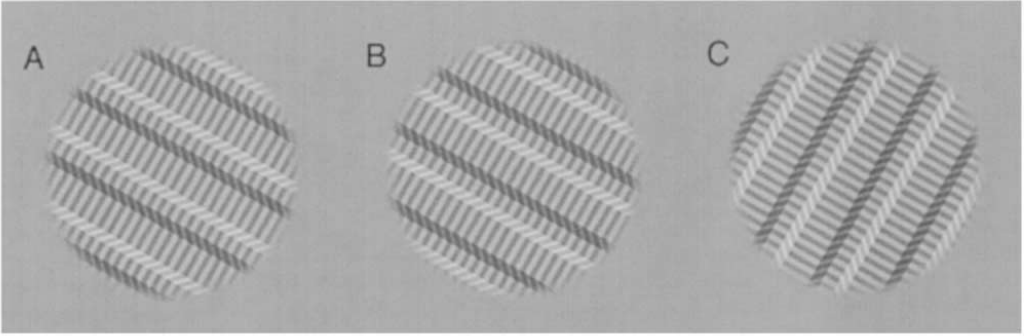
\includegraphics[scale=0.5]{Mamassian2001a(1).png}
		\caption{Ejemplos de estímulos usados en la tarea.}
	\end{center}
\end{figure}

El contraste entre las partes oscuras y claras en los contornos paralelos era constante e igual al {\itshape contour contrast}, $C_{C}$. Estos contrastes eran entonces
\begin{equation}
	C_{S}
	=
	\frac{
		B_{3}-B_{2}
	}{
		B_{3}+B_{2}
	}
	=
	\frac{
		B_{2}-B_{1}
	}{
		B_{2}+B_{1}
	}
	=
	\frac{
		D_{3}-D_{2}
	}{
		D_{3}+D_{2}
	}
	=
	\frac{
		D_{2}-D_{1}
	}{
		D_{2}+D_{1}
	}
\end{equation}
y
\begin{equation}
	C_{C}
	=
	\frac{
		B_{1}-D_{1}
	}{
		B_{1}+D_{1}
	}
	=
	\frac{
		B_{2}-D_{2}
	}{
		B_{2}+D_{2}
	}
	=
	\frac{
		B_{3}-D_{3}
	}{
		B_{3}+D_{3}
	},
\end{equation}
donde $B_{1}, B_{2},$ y $B_{3}$ son las intensidades sobre os contornos paralelos claros, y $D_{1}, D_{2}$ y $D_{3}$ son las intensidades sobre los contornos oscuros. $C_{S}$ se deriva de las cantidades relativas de fuente e iluminación ambiental, y $C_{C}$ es el contraste entre las dos reflectividades de superficie correspondientes a los contornos claros y oscuros. Hubo 3 niveles de $C_{S}$ y 3 de $C_{C}$, lo que llevó a 9 condiciones de contraste. Y como contrabalanceo se utilizó una reflexión especular de cada estímulo para un total de 18 estímulos (figura 2).

\begin{figure}[hb]
	\begin{center}
		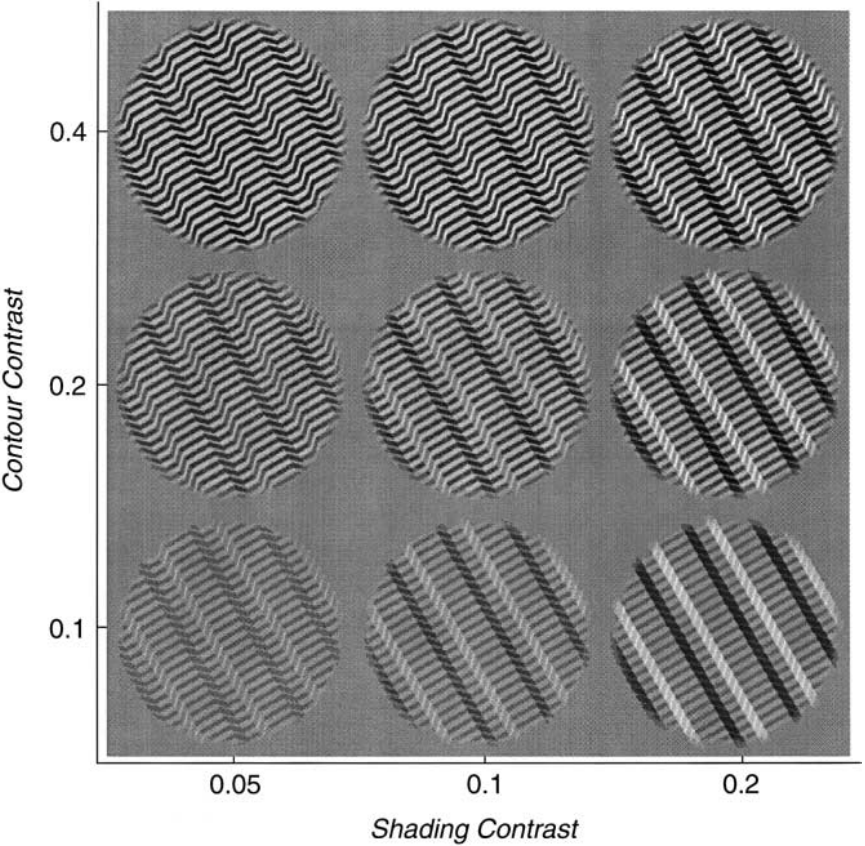
\includegraphics[scale=0.5]{Mamassian2001a(2).png}
		\caption{La mitad de los estímulos utilizados (la otra mitad son sus reflexiones especulares).}
	\end{center}	
\end{figure}

Cada estímulo se presentó en 24 orientaciones distintas.

La tarea del observador era decidir si el percepto inicial era de una superficie en relieve con barras anchas o angostas en altorrelieve. Respondían con las teclas de una teclado.

{\scshape\bfseries Results}

Los resultados se presentan en términos del {\itshape narrow score}, la proporción de ocasiones en que el patrón fue percibido como barras estrechas en altorrelieve. Un mismo estímulo en distintos ángulos de rotación podía llevar a perceptos distintos (figura 3). Las tres orientaciones de la figura 1 se resaltan en la gráfica y se muestra que llevaron a un puntaje alto, uno bajo, y uno azaroso a pesar de tratarse de un único estímulo en distintas orientaciones.

\begin{figure}[ht]
	\begin{center}
		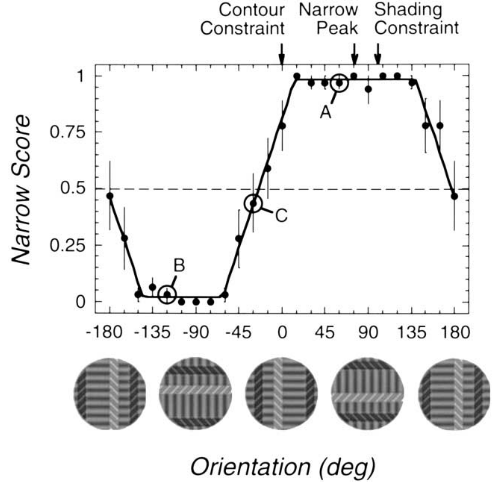
\includegraphics[scale=0.5]{Mamassian2001a(3).png}
		\caption{Resultados de {\itshape narrow score} de la figura 1.}
	\end{center}
\end{figure}

También se presentan los puntos predichos para los puntajes más altos de {\itshape narrow score} de acuerdo con cada restricción (es decir, el punto en el que la limitación sería más efectiva y por lo tanto sesgaría en mayor medida el percepto). En los datos reales el pico cayó en medio de los dos picos predichos.

Se muestra la misma gráfica para cada uno de los estímulos utilizados. Cada gráfica contiene los datos de las dos reflexiones especulares de su estímulo correspondiente (figura 4).

\begin{figure}[ht]
	\begin{center}
		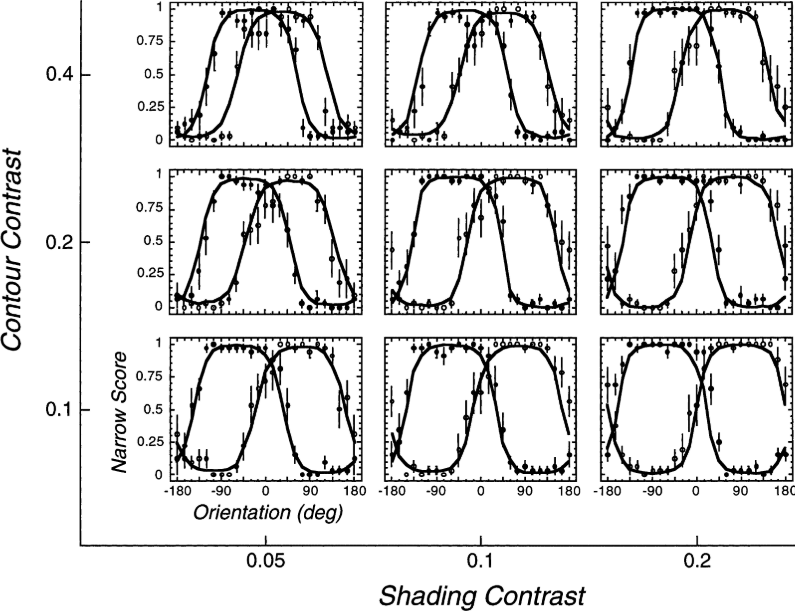
\includegraphics[scale=0.5]{Mamassian2001a(4).png}
		\caption{Resultados de todos los estímulos.}
	\end{center}
\end{figure}

Se observa un cambo sistemático en el pico del {\itshape narrow score} en ambas curvas mientras el contraste relativo cambia de uno que favorece al uso de los contornos (gráfica de arriba a la izquierda) a uno que favorece el uso del sombreado (abajo a la derecha).

Se estimaron las orientaciones que llevaban al pico en el {\itshape narrow score} para cada condición. La función que lo captura se compone de un rango para el desempeño de piso, un incremento lineal, un rango para el techo, y un decremento lineal. La curva se ajustó mediante mínimos cuadrados.

{\scshape\bfseries Discussion}

Cuando las restricciones son consistentes, el sistema visual las usa en forma cooperativa. Cuando no, la probabilidad de elegir uno sobre el otro depende de la calidad de la información del estímulo dada por la clave correspondiente a cada limitación. Esto es similar a la alocación dinámica de pesos para claves sensoriales.

A continuación se provee un método para determinar cuantitativamente los pesos asignados a cada restricción. Se desarrolla un modelo para la tarea y luego se ajusta a los datos observados. Esto permitirá relacionar la forma de la distribución de priors con las restricciones de {\itshape shading} y {\itshape contour}.

{\scshape\bfseries Models}

El propósito de los modelos es entender el principio por el que interactúan las dos restricciones. 

{\scshape Overview of the approach}

Similar a los modelos Bayesianos, tiene tres componentes: (1) cálculo de la función de verosimilitud (probabilidad de que ciertos datos sensoriales sean observados dado que el mundo está en un estado $X$); (2) una descripción de las restricciones en términos de funciones de distribución de priors; y (3) una regla de decisión. Se combinan de forma óptima los datos sensoriales con los priors, y la regla de decisión enlaza este resultado con los datos observados.

La función de verosimilitud se puede expresar solo bajo el costo de hacer explícitos todos los atributos de la escena que pueden influir en la apariencia de la imagen, por lo que se modelará la iluminación, forma de la superficie y orientación. Otras variables aleatorias que puedan interferir serán asumidas como distribuciones uniformes.

Habrá tres restricciones prior: (1) la luz proviene de una dirección preferida ({\itshape shading constraint}); (2) restricción en la orientación de la superficie ({\itshape contour constraint}); y (3) un sesgo general a percibir ``angosto'' en lugar de ``ancho''.

Como regla de decisión se usará una regla no determinista para capturar la variabilidad de los juicios de los humanos. La regla será {\itshape non-committing} e igualará la probabilidad de responder ``{\itshape narrow}'' será igual a la probabilidad posterior del modelo.

{\scshape Bayesian combination}

Con base en las distribuciones propuestas para las restricciones se puede computar la función de verosimilitud $p(image|scene)$, que refleja la probabilidad de que una imagen sea una proyección de una escena. La escena se reduce a la propiedad de que la superficie tenga barras angostas o anchas en altorrelieve. La imagen corresponde a las variables independientes del experimento, es decir, la combinación de {\itshape shading contrast} $C_{S}$, {\itshape contour contrast} $C_{C}$, ángulo proyectado por el bisel (siempre 45° en este caso), y orientación de la figura en el plano frontal. Se computa la verosimilitud mediante el principio de probabilidad total para incluir todos los parámetros que apliquen, y se computa la probabilidad posterior usando el teorema de Bayes.

{\scshape The full model in a nutshell}

Se desarrolló un modelo que incluye aspectos del análisis Bayesiano para la tarea psicofísica. El modelo tiene cuatro parámetros: (1) sesgo para preferir superficies con barras angostas sobresalientes, (2) sesgo en la inclinación de la dirección de la luz, (3) parámetro de concentración para la inclinación de la dirección de la luz, y (4) parámetro de concentración para la inclinación de la superficie.

{\scshape Results}

El modelo tiene 20 parámetros. Se ajustó a los 432 datos (24 orientaciones $\times$ 9 combinaciones de contraste $\times$ 2 reflejos especulares) usando el método {\itshape downhill simplex} para encontrar el ajuste de máxima verosimilitud. 

Se encontró un buen ajuste del modelo a los datos. Como se esperaban, se encontró un sesgo para responder ``angosto'' por encima de ``ancho'' y un seso para asumir que la luz proviene ligeramente a la izquierda de la vertical.

{\scshape Intermediate discussion}

Hay tres formas en que este modelo se diferencia de modelos Bayesianos más tradicionales.

\begin{enumerate}
	\item La función de verosimilitud era determinista y binaria en lugar de estocástica y continua. Las fuentes de ruido limitan la percepción del estímulo. Dado el ruido, un mismo estímulo distal puede producir una distribución de estímulos proximales. El ruido afecta el mapeo de estados del mundo real a atributos de imagen. En los modelos descritos hasta ahora se a menospreciado el ruido del ambiente. Suponiendo que tanto el ruido en los juicios del observador como el ruido de los estímulos mismos eran pequeños se llegó a la construcción de una función de verosimilitud binaria y determinista: o la imagen era consistente con una descripción dada del mundo o no lo era.
	\item Lo segundo es la manera en que se trata a los priors. Se ha resaltado que la ambigüedad inherente a todos los estímulos proximales solo puede sobrepasarse gracias a las restricciones. Así, parece natural pensar en los priors como fuentes de información independientes de los estímulos. En este modelo se han representado las distribuciones de priors como funciones de dos parámetros: la media y la varianza de una distribución de probabilidad. 
	\item Finalmente, un modelo Bayesiano real escogería primero una función de ganancia que recompensa máximamente una respuesta ``correcta'', por lo que tendría que usar una regla de decisión que maximice la ganancia esperada. Es importante que todas las reglas de decisión Bayesianas son deterministas, mientras que la variabilidad se encuentra en el ruido. En este caso se incorporó la variabilidad al nivel de la regla de decisión usando una regla no-comprometedora. Mientras las reglas de decisión Bayesianas son óptimas, la regla no comprometedora es subóptima pero probablemente más realista.
\end{enumerate}

{\scshape\bfseries General discussion}

Los resultados de este experimento psicofísico muestran una clara interacción entre dos restricciones visuales en la interpretación de estímulos ambiguos. Se propusieron modelos inspirados en modelos de decisión Bayesianos para capturar el desempeño de los humanos (en este resumen solo hay uno descrito, pero se propusieron tres).

Una alternativa al modelamiento de conductas psicológicas es usar modelos Thrustonianos basados en fuerza. Para un modelo así se tendría que elegir un conjunto de funciones paramétricas para describir la contribución de cada restricción para la interpretación de los estímulos. Cada función caracterizaría la fuerza de una sola restricción asumiendo que las otras no hacen ninguna contribución, de modo que la interacción de las dos restricciones se modelaría como la combinación ponderada de las fuerzas de las restricciones individuales. Aunque estos datos podrían modelarse con un modelo así, los autores piensan que la aproximación usada tiene varias ventajas: (1) el modelo fue construido siguiendo principios y basándose en propiedades físicas (geometría, iluminación) y componentes psicológicos. Como resultado la regla de combinación para las restricciones no se imponía por el modelador, sino que emergía naturalmente del proceso de modelado. Esto permitía estudiar la interacción a posteriori. (2) La segunda ventaja está en la interpretación de los parámetros. Dado que no hay componentes {\itshape ad hoc} en el modelo, cada parámetro tiene un significad claro, lo que permite hacer predicciones cuantitativas.

{\scshape Scope of the study}

Este estudió se enfocó en la primera interpretación de estímulos ambiguos. Se pensó que si las restricciones tenían un efecto, este aparecería al inicio del procesamiento del estímulo. Se encontró un efecto significativo de las restricciones visuales en la interpretación de los estímulos.

En este caso el estímulo desaparecía de inmediato tras emitir un juicio, cuando es sabido que ante estímulos ambiguos y dado suficiente tiempo las interpretaciones comienzan a alternar. Se predice que el período en que se percibiría cada percepto es proporcional a la probabilidad posterior de cada uno. Por lo tanto, las restricciones prior no son útiles solamente para la primera interpretación, sino que permanece siéndolo en tanto el estímulo sea observado.

{\scshape Summary}

Se encontró que la interpretación de un estímulo ambiguo elegida por un observador es efectivamente un compromiso (en sentido probabilístico) entre lo indicado por dos restricciones que gobiernan dos claves de profundidad presentes en los estímulos. Cuando la información para una clave era más confiable que para otra, entonces la restricción correspondiente predominaba.

\end{document}
